%% bare_jrnl.tex
%% V1.3
%% 2007/01/11
%% by Michael Shell
%% see http://www.michaelshell.org/
%% for current contact information.
\documentclass[journal]{IEEEtran}


\usepackage{graphicx}
\usepackage{geometry}
\usepackage{epstopdf}

% *** MATH PACKAGES ***
%
\usepackage[cmex10]{amsmath}
% A popular package from the American Mathematical Society that provides
% many useful and powerful commands for dealing with mathematics. If using
% it, be sure to load this package with the cmex10 option to ensure that
% only type 1 fonts will utilized at all point sizes. Without this option,
% it is possible that some math symbols, particularly those within
% footnotes, will be rendered in bitmap form which will result in a
% document that can not be IEEE Xplore compliant!
%
% Also, note that the amsmath package sets \interdisplaylinepenalty to 10000
% thus preventing page breaks from occurring within multiline equations. Use:
%\interdisplaylinepenalty=2500
% after loading amsmath to restore such page breaks as IEEEtran.cls normally
% does. amsmath.sty is already installed on most LaTeX systems. The latest
% version and documentation can be obtained at:
% http://www.ctan.org/tex-archive/macros/latex/required/amslatex/math/

% *** SPECIALIZED LIST PACKAGES ***
%
\usepackage{algorithmic}
% algorithmic.sty was written by Peter Williams and Rogerio Brito.
% This package provides an algorithmic environment fo describing algorithms.
% You can use the algorithmic environment in-text or within a figure
% environment to provide for a floating algorithm. Do NOT use the algorithm
% floating environment provided by algorithm.sty (by the same authors) or
% algorithm2e.sty (by Christophe Fiorio) as IEEE does not use dedicated
% algorithm float types and packages that provide these will not provide
% correct IEEE style captions. The latest version and documentation of
% algorithmic.sty can be obtained at:
% http://www.ctan.org/tex-archive/macros/latex/contrib/algorithms/
% There is also a support site at:
% http://algorithms.berlios.de/index.html
% Also of interest may be the (relatively newer and more customizable)
% algorithmicx.sty package by Szasz Janos:
% http://www.ctan.org/tex-archive/macros/latex/contrib/algorithmicx/



% *** SUBFIGURE PACKAGES ***
\usepackage[tight,footnotesize]{subfigure}
% subfigure.sty was written by Steven Douglas Cochran. This package makes it
% easy to put subfigures in your figures. e.g., "Figure 1a and 1b". For IEEE
% work, it is a good idea to load it with the tight package option to reduce
% the amount of white space around the subfigures. subfigure.sty is already
% installed on most LaTeX systems. The latest version and documentation can
% be obtained at:
% http://www.ctan.org/tex-archive/obsolete/macros/latex/contrib/subfigure/
% subfigure.sty has been superceeded by subfig.sty.



\begin{document}
%
% paper title
% can use linebreaks \\ within to get better formatting as desired
\title{Face recognition}

\author{Axel Beauvisage, Carole Belloni, Adrian Kostkowski, Gareth Hughes, Domonkos Huszar}

% The paper headers
\markboth{Image Analysis group project, March~2015, Cranfield University}{}
% The only time the second header will appear is for the odd numbered pages
% after the title page when using the twoside option.

\maketitle


\begin{abstract}
%\boldmath
The abstract goes here.
\end{abstract}
% IEEEtran.cls defaults to using nonbold math in the Abstract.
% This preserves the distinction between vectors and scalars. However,
% if the journal you are submitting to favors bold math in the abstract,
% then you can use LaTeX's standard command \boldmath at the very start
% of the abstract to achieve this. Many IEEE journals frown on math
% in the abstract anyway.


\IEEEpeerreviewmaketitle



\section{Introduction}
% The very first letter is a 2 line initial drop letter followed
% by the rest of the first word in caps.
% 
% form to use if the first word consists of a single letter:
% \IEEEPARstart{A}{demo} file is ....
% 
% form to use if you need the single drop letter followed by
% normal text (unknown if ever used by IEEE):
% \IEEEPARstart{A}{}demo file is ....
% 
% Some journals put the first two words in caps:
% \IEEEPARstart{T}{his demo} file is ....
% 
% Here we have the typical use of a "T" for an initial drop letter
% and "HIS" in caps to complete the first word.
\IEEEPARstart{T}{his} demo file is intended to serve as a ``starter file''
for IEEE journal papers produced under \LaTeX\ using
IEEEtran.cls version 1.7 and later.
% You must have at least 2 lines in the paragraph with the drop letter
% (should never be an issue)
I wish you the best of success.

\hfill mds
 
\hfill January 11, 2007

\subsection{Subsection Heading Here}
Subsection text here.

\subsubsection{Subsubsection Heading Here}
Subsubsection text here.


% An example of a floating figure using the graphicx package.
% Note that \label must occur AFTER (or within) \caption.
% For figures, \caption should occur after the \includegraphics.
% Note that IEEEtran v1.7 and later has special internal code that
% is designed to preserve the operation of \label within \caption
% even when the captionsoff option is in effect. However, because
% of issues like this, it may be the safest practice to put all your
% \label just after \caption rather than within \caption{}.

% example figure
\begin{figure}[!t]
\centering
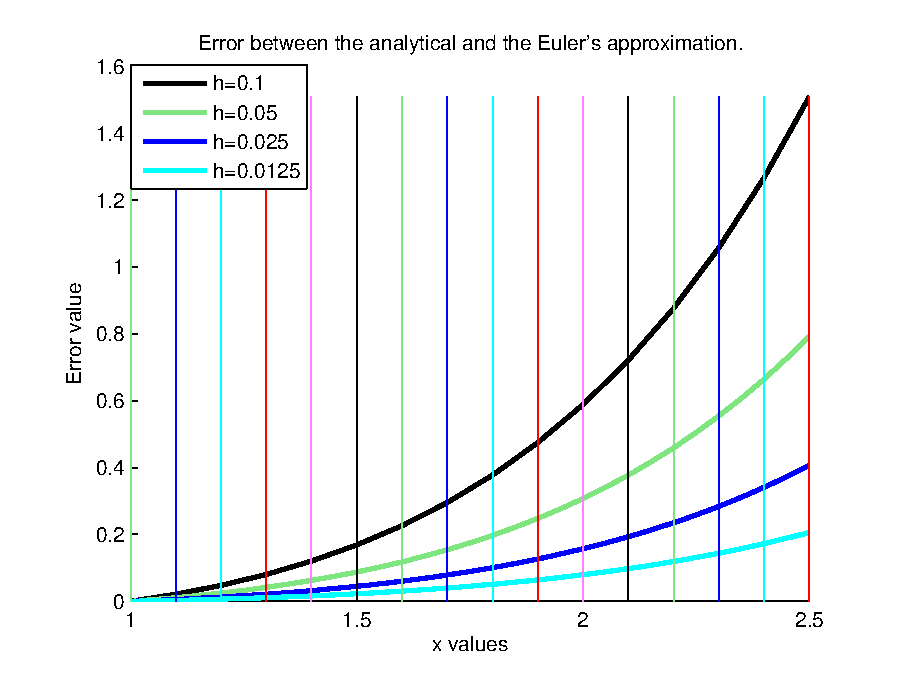
\includegraphics[width=2.5in]{rsrc/example.eps}
\caption{Simulation Results}
\label{fig_sim}
\end{figure}

\section {Methods}
\subsection{Fisher method}
\begin{figure}
	\centering		
	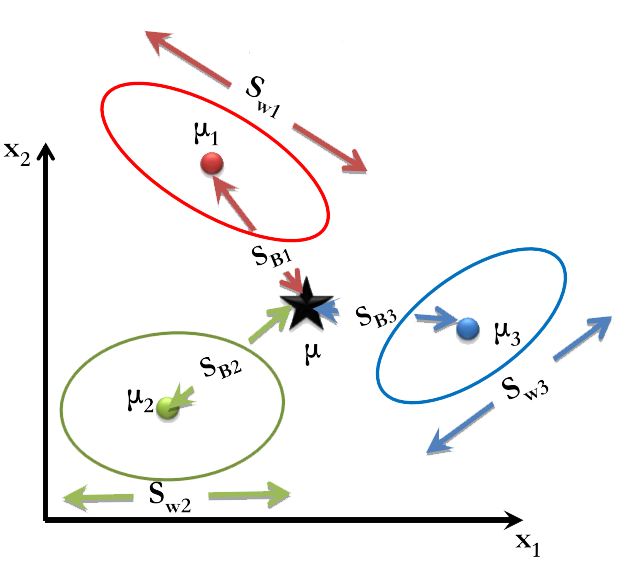
\includegraphics[width = 0.4\textwidth]{rsrc/LDA_basic.png}
	\caption{Az LDA algoritmus által megvizsgált szórások. The source of the image: \cite{LDA}}
	\label{fig:LDA abrazolas}
\end{figure}

Ha $ m $ dimenziós vektorokat szeretnék leképezni egy $ C $-dimenziós térbe akkor azt a következő módon tehetem meg.
\begin{equation}
y = w^Tx \textrm{, where } 
\end{equation}
\begin{equation}
x = \left(
\begin{array}{ccc}
x_1\\
\vdots\\
x_m
\end{array} \right)
w=\left(
\begin{array}{ccc}
w_{1,1} \dots w_{1,C}\\
\vdots \ddots \vdots\\
w_{m,1} \dots w_{m,C}
\end{array}
\right)
y = \left(
\begin{array}{ccc}
y_1\\
\vdots\\
y_C
\end{array}\right)
\label{equ:Alap_egyenlet}
\end{equation}

\section {Implementation}

\section{Results}

\section{Conclusion}
The conclusion goes here.


\appendices
\section{Proof of the First Zonklar Equation}
Appendix one text goes here.

% you can choose not to have a title for an appendix
% if you want by leaving the argument blank
\section{Important code parts}
Appendix two text goes here.


% use section* for acknowledgement
\section*{Acknowledgement}


The authors would like to thank...


%\begin{thebibliography}{1}

%\bibitem{IEEEhowto:kopka}
%H.~Kopka and P.~W. Daly, \emph{A Guide to \LaTeX}, 3rd~ed.\hskip 1em plus
%  0.5em minus 0.4em\relax Harlow, England: Addison-Wesley, 1999.
  
%\end{thebibliography}

\bibliographystyle{IEEEtran}
\bibliography{rsrc/bibliography} % adjust this to fit your BibTex file

% that's all folks
\end{document}


